\section{EXPERIMENT 1: DISCRIMINATING DIRECTION OF RESULTANT FORCES}

%In this experiment, we evaluated whether the direction of the resultant force from the device was perceived correctly.
In this experiment, we evaluated whether the direction of the tangential force presented by the device was perceived correctly.
Participants answered the direction of force either left or right.
%The experiment was designed by following a just noticeable differences (JND) methodology~\cite{gescheider1985psychophysics}. 
The experiment was performed by a constant method, and a psychometric curve was obtained as a result of discriminating the direction perceived by the participants.

\subsection{Experimental Environment}

Participants sat on a chair, and they wore either 45$^{\circ}$ or 60$^{\circ}$ device on their fingertip of the dominant hands'{} thumb. 
During the experiment, participants wore the headphone with noise canceling function, and environmental noise was blocked by white noise from the headphone.
Fig.\ref{fig_ex1_environment} shows an experimental environment of experiment 1. 
The number of participants was eight (six males and two females, aged between 22 to 26).

\begin{figure}[h]
  \centering
  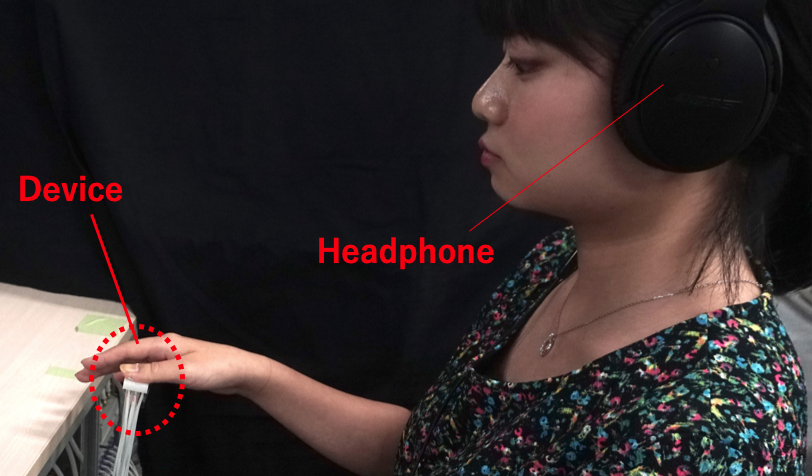
\includegraphics[width=3.4in]{images/fig_ex1_environment.png}
  \caption{Experimental environment of the experiment 1.}
  \label{fig_ex1_environment}
\end{figure}

\subsection{Standard Stimulus and Comparison Stimuli}

Standard stimulus was the stimulus when $\theta$ was 0$^{\circ}$ in expression (\ref{eq:theta}). % 圧力がどれくらいだったかの記述が必要
% A. 式(1)の結果が1Nになるように圧力を決定
% 標準刺激の場合は45dデバイスで0.116Mpa, 60dデバイスで0.120Mpaですね.→ありがとうございます!
%The pressure output to each pin of the standard stimulus was 0.116 Mpa for the 45$^{\circ}$ device and 0.120 Mpa for the 60$^{\circ}$ device.
%These values were configured so that the intensity of the resultant force in expression (\ref{eq:1}) equaled to 1N.
 The pressure output $F_{R}$ and $F_{L}$ were designed so that the resultant force in expression (\ref{eq:1}) equaled to 1N.

On the other hand, the comparison stimulus was the stimulus $\theta$ of which was every 5$^{\circ}$ from the limit angle that each device can present. 
In the case of the 45$^{\circ}$ device, the comparison stimulus was the ones when $\theta$ was from +45$^{\circ}$ to -45$^{\circ}$. 
In the case of 60$^{\circ}$ device, the comparison stimulus was the ones when $\theta$ was from +60$^{\circ}$ to -60.
% As the angle of the force of the presentation stimulus tilts from 0$^{\circ}$, the direction becomes easier to perceive.
% Therefore, it is considered that the correct answer rate becomes higher as the angle becomes larger. % ここに仮説を書くかはあとで考える。

\subsection{Task Design}

For each trial, participants performed
the standard stimulus and the comparison stimulus sequentially, and they stated whether the direction of the tangential force presented from the device was "left" or "right". % 刺激した時間ってどのくらい?
% A. 標準刺激は約1秒くらい提示しました.
%    比較刺激の方は被験者が答えるまで無制限で出してました.
%    大体の被験者は2,3秒で答えてましたが,たまに迷った時は5秒くらいかかってたときもありました.
%    ただ時間的な記録が残っていないので,無制限としか書けないですね.
Standard stimulus was presented for about 1 second.
The comparison stimulus continued to be presented until participants answered.

For each comparison stimulus, the participant answered 5 times. % 試行回数いくつだっけ
%A. 5回です.
With 45$^{\circ}$ device, the number of comparison stimuli was 18 and thus, the total number of trials per participant was 90. 
With 60$^{\circ}$ device, the number of comparison stimuli was 24 and thus, the total number of trials per participant was 120. % 広田先生に冗長といわれるかも
The order of comparison stimuli was randomly assigned.
In addition, whether participants wore 45$^{\circ}$ or 60$^{\circ}$ device first was assigned to the participant to be counter-balanced.

\subsection{Results}

Fig.\ref{fig_jnd_45} and Fig.\ref{fig_jnd_60} show the average value of the probability that the participants answered “right”. 
Error bars represent standard error. 
The ratio of answering “right” increased as the angle leaned further to right in both devices. 
%In order to investigate the subjective equivalent point and the discrimination thresholds for clearly recognizing the difference in angles, the least-squares fitting was performed using a cumulative normal distribution function, which is shown in the orange line in Fig.\ref{fig_jnd_45} and Fig.\ref{fig_jnd_60}.
In order to obtain a psychometric curve, the least-squares fitting was performed using a cumulative normal distribution function, which is shown in the orange line in Fig. \ref{fig_jnd_45} and Fig. \ref{fig_jnd_60}.
The point of subjective equality (PSE), which represents the value of evaluation stimulus judged as “equal to the standard stimulus”, was +3.1$^{\circ}$ in the 45$^{\circ}$ device and +4.3$^{\circ}$ in the 60$^{\circ}$ device. 
The just-noticeable difference (JND) representing “the minimum difference between 2 stimuli discrimination with a confidence rate of 50\% of the judgment number” was 46.5$^{\circ}$ in the 45$^{\circ}$ device and 36.4$^{\circ}$ in the 60$^{\circ}$ device.

\begin{figure}[h]
  \centering
  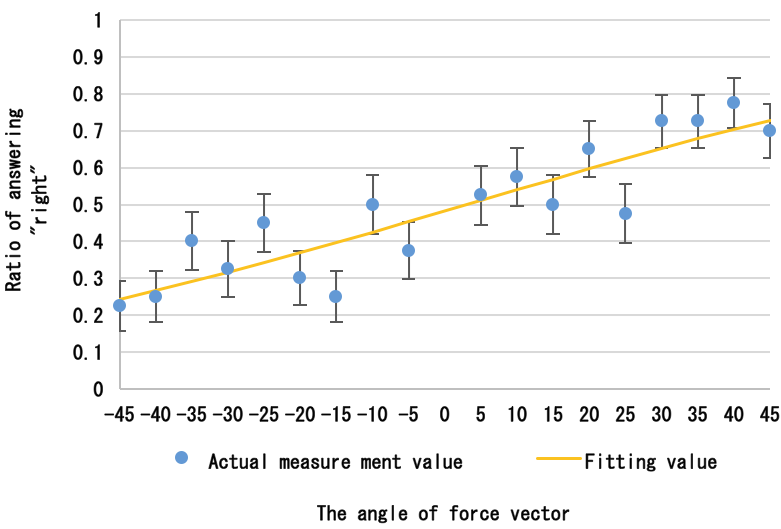
\includegraphics[width=3.4in]{images/fig_jnd_45.png}
  \caption{The ratio of participants answer "right" with the 45$^{\circ}$ device.}
  \label{fig_jnd_45}
\end{figure}

\begin{figure}[h]
  \centering
  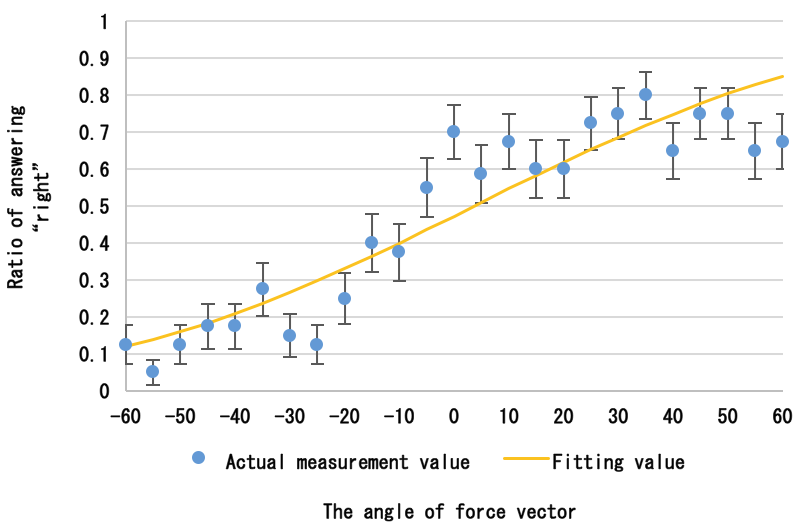
\includegraphics[width=3.4in]{images/fig_jnd_60.png}
  \caption{The ratio of participants answer "right" with the 60$^{\circ}$ device.}
  \label{fig_jnd_60}
\end{figure}

\subsection{Discussion}
%According to the result, participants discriminated the direction of resultant force at approximately 75\% at maximum with 45$^{\circ}$ device and 85\% at maximum with 60$^{\circ}$ device.
%Thus, the discrimination performance was better with 60$^{\circ}$ device than 45$^{\circ}$ device.
%The comparison between the JND value suggests the same conclusion.
%This is reasonable because the cosine term becomes large when $d$ is large in expression (\ref{eq:1}).

%被験者ごとのJNDをt検定で比較したが有意差なし
In this experiment, the JND of the 60$^{\circ}$ device was smaller than 45$^{\circ}$ device.
To determine whether there is a difference in the JND of two conditions, we performed the t-test obtained from each participants'{} JND values.
However, there was no significant difference.

%To realize better performance, the increase in the pin's inclination angle is one option.

%有意差はないが,60dデバイスの方が提示可能な刺激の角度が30度多い.
%(左右に15度ずつ)
%そのため,ピンの傾斜角を増加させることは,提示可能な刺激の自由度を高めることにつながる.
%Although there was no significant difference in the JND, 60$^{\circ}$ device can present 30$^{\circ}$ (15$^{\circ}$ left and right) larger angles than the 45$^{\circ}$ device.
There was no significant difference in the JND which suggests that the 60d device is a better implementation in that it can prezent the force of wider angle range.
Thus, increasing the pin's inclination angle will increase the degree of felt inclination of the angle of the resultant force that the device can present.

Another option to increase the felt inclination angle of the resultant force will be to increase the number of pins or applied pressure.
We should flexibly change these parameters based on design constraints to realize better recognition performance.

Overall, we showed that there is a possibility that participants can recognize the direction of the resultant force with the proposed device.